\documentclass[11pt]{article}

\usepackage{amsfonts}
\usepackage{graphicx}

%\VignetteIndexEntry{Multivariable Fractional Polynomials}
%\VignetteKeywords{variable selection, transformation, regression, fractional polynomials}
%\VignetteDepends{mfp}

%\renewcommand{\figurename}{\footnotesize Figure}
%\renewcommand{\tablename}{\footnotesize Table}

\setlength{\parindent}{0pt}
\setlength{\oddsidemargin}{-0,5cm}
\setlength{\textwidth}{17cm}
\setlength{\topmargin}{-1,7cm}
\setlength{\textheight}{23.5cm}

\usepackage{/Library/Frameworks/R.framework/Resources/share/texmf/Sweave}
\begin{document}

\title{Multivariable Fractional Polynomials}
\author{Axel Benner}




\maketitle
\tableofcontents
\section{Introduction}
The \texttt{mfp} package is a collection of R \cite{R04} functions targeted at the use of fractional polynomials (FP) for modelling the influence of continuous covariates on the outcome in regression models, as introduced by Royston \&\ Altman (1994) \cite{FP94} and 
modified by Sauerbrei \&\ Royston (1999) \cite{SauRoy99}. 
The model may include binary, categorical or further continuous covariates which are included in the variable selection process but without need of FP transformation.
It combines backward elimination with a systematic search for a `suitable' transformation 
to represent the influence of each continuous covariate on the outcome. 
An application of multivariable fractional polynomials (MFP) in modelling prognostic and 
diagnostic factors in breast cancer is given by \cite{SauRoy99}.
The stability of the models selected is investigated in \cite{RoySau03}.
Briefly, fractional polynomials models are useful when one wishes to preserve the continuous 
nature of the covariates in a regression model, but suspects that some or all of the 
relationships may be non-linear. 
At each step of a `backfitting' algorithm MFP constructs a fractional polynomial transformation
for each continuous covariate while fixing the current functional forms of the other covariates. 
The algorithm terminates when no more covariate is excluded and the functional forms of the continuous covariates do not change anymore.

\section{Inventory of functions}

\texttt{mfp.object} is an object representing a fitted \texttt{mfp} model. 
Class \texttt{mfp} inherits from either glm or coxph depending on the type of model fitted.
In addition to the standard glm/coxph components the following components are included in an 
\texttt{mfp} object
\begin{description}
\item[x]  
the final FP transformations that are contained in the design matrix x. 
The covariate "z" with 4 df (second-degree FP) has corresponding columns "z.1" and "z.2" in x.
A first-degree FP covariate "z" would have one column "z.1".
\item[powers]  
a matrix containing the best FP powers for each covariate. 
If a covariate has less than two powers NAs will fill the appropriate cell of the matrix.
\item[pvalues]     
a matrix containing the P-values from the ''closed test procedure'' together with the best powers chosen. 
Briefly p.null is the P-value for the test of inclusion (see mfp), p.lin corresponds to the 
test of nonlinearity and p.FP the test of simplification by comparing first degree (FP1) and second degree (FP2) transformations. 
The best first degree FP power (power2) and best second degree FP powers (power4.1 and power4.2) are also given. The numbers 2 and 4 describe the corresponding degrees of freedom.
\item[scale]   
all covariates are shifted and rescaled before being power transformed if nonpositive values 
are encountered or the range of values of the covariates is reasonably large. 
If x' would be used instead of x where x' = (x+a)/b the parameters a (shift) and b (scale) 
are contained in the matrix scale.
\item[df.initial]  
a vector containing the degrees of freedom allocated to each covariate corresponding to the degree of FP (m=4 for second degree FP, m=2 for first degree FP).
\item[df.final]    
a vector containing the degrees of freedom of each covariate at convergence of the backfitting 
algorithm (m=4 for second degree FP, m=2 for first degree FP, m=1 for untransformed variable, m=0 if covariate was excluded).
\item[dev]     
the deviance of the final model.
\item[dev.lin]     
the deviance of the model that uses the linear predictor of untransformed  covariates.
\item[dev.null]    
the deviance of the null model.
\item[fptable]     
the table of the final fp transformations.
\item[fit]     
a call of the corresponding glm or cox model using the selected and (possibly) FP  transformed variables of the final model.
\end{description}

\section{Usage in R}

Start with

\begin{Schunk}
\begin{Sinput}
>library(mfp)
\end{Sinput}
\end{Schunk}

An \texttt{mfp.object} will be created by application of function \texttt{mfp}. 

A typical call of an mfp model has the form \texttt{response $\sim$ terms} where \texttt{response} is the 
(numeric) response vector and \texttt{terms} is a series of terms, separated by $+$ operators,
which specifies a linear predictor for \texttt{response} provided by the \texttt{formula} 
argument of the function call.

\begin{Schunk}
\begin{Sinput}
>str(mfp)
\end{Sinput}
\begin{Soutput}
function (formula = formula(data), data = parent.frame(), family = gaussian, 
    method = c("efron", "breslow"), subset = NULL, na.action = na.omit, 
    init = NULL, alpha = 0.05, select = 1, maxits = 20, keep = NULL, 
    rescale = TRUE, verbose = FALSE, x = TRUE, y = TRUE)  
\end{Soutput}
\end{Schunk}

Fractional polynomial terms are indicated by \texttt{fp}. 

For \texttt{binomial} models the response can also be specified as a \texttt{factor}. 
If a Cox proportional hazards model is required then the outcome need to be specified using 
the \texttt{Surv()} notation. 

The argument \texttt{family} describes the error distribution and link function to
be used in the model. 
This can be a character string naming a family function, a family function or the result 
of a call to a family function. 

Argument \texttt{alpha} sets the global FP selection level for all covariates. 
Different selection levels for individual covariates can be chosen by using the \texttt{fp} function.
The variable selection level for all covariates is set by \texttt{select}. 
Values for individual fractional polynomials may be set using the \texttt{fp} function.

The function \texttt{fp} defines a fractional polynomial object for a single input 
variable. 

\begin{Schunk}
\begin{Sinput}
>str(fp)
\end{Sinput}
\begin{Soutput}
function (x, df = 4, select = NA, alpha = NA, scale = TRUE)  
\end{Soutput}
\end{Schunk}

In addition to \texttt{alpha} and \texttt{select} the \texttt{scale} argument of the 
\texttt{fp} function denotes the use of pre-transformation scaling to avoid possible 
numerical problems or for variables with non-positive values.

\subsection{Model selection}
The original Stata implementation of \texttt{mfp} uses two different selection procedures
for a single continuous covariate $x$, a sequential selection procedure and a closed 
testing selection procedure ({\tt ra2},  \cite{AmbRoy01} ).
In the R implementation only the {\tt ra2} algorithm is used which is also the default in the Stata and SAS implementations of \texttt{mfp}. 
 
The {\tt ra2} algorithm is described in \cite{AmbRoy01} and \cite{SauRoy02}. 
It uses a closed test procedure \cite{MarPerGab76} which maintains 
approximately the correct Type I error rate for each component test. 
The procedure allows the complexity of candidate models to increase progressively from a 
prespecified minimum (a null model) to a prespecified maximum (an FP) according to an 
ordered sequence of test results.

The algorithm works as follows:
\begin{enumerate}
\item Perform a 4 df test at the $\alpha$ level of the best-fitting second-degree FP against 
the null model. 
If the test is not significant, drop $x$ and stop, otherwise continue.
\item Perform a 3 df test at the $\alpha$ level of the best-fitting second-degree FP against 
a straight line. 
If the test is not significant, stop (the final model is a straight line), otherwise continue.
\item Perform a 2 df test at the $\alpha$ level of the best-fitting second-degree FP against 
the best-fitting first-degree FP. 
If the test is significant, the final model is the FP with $m=2$, otherwise the FP with $m=1$. 
\end{enumerate}
The tests in step 1, 2 and 3 are of overall association, non-linearity and between a simpler 
or more complex FP model, respectively.

\section{Example}
\subsection{Cox proportional hazards model}
We use the dataset \texttt{GBSG} which contains data from a study of the German Breast Cancer Study Group for patients with node-positive breast cancer. 
\begin{Schunk}
\begin{Sinput}
>data(GBSG)
>str(GBSG)
\end{Sinput}
\begin{Soutput}
'data.frame':	686 obs. of  11 variables:
 $ id      : int  1 2 3 4 5 6 7 8 9 10 ...
 $ htreat  : Factor w/ 2 levels "0","1": 1 2 2 2 1 1 2 1 1 1 ...
 $ age     : int  70 56 58 59 73 32 59 65 80 66 ...
 $ menostat: Factor w/ 2 levels "1","2": 2 2 2 2 2 1 2 2 2 2 ...
 $ tumsize : int  21 12 35 17 35 57 8 16 39 18 ...
 $ tumgrad : Factor w/ 3 levels "1","2","3": 2 2 2 2 2 3 2 2 2 2 ...
 $ posnodal: int  3 7 9 4 1 24 2 1 30 7 ...
 $ prm     : int  48 61 52 60 26 0 181 192 0 0 ...
 $ esm     : int  66 77 271 29 65 13 0 25 59 3 ...
 $ rfst    : int  1814 2018 712 1807 772 448 2172 2161 471 2014 ...
 $ cens    : int  1 1 1 1 1 1 0 0 1 0 ...
\end{Soutput}
\end{Schunk}

The response variable is recurrence free survival time ({\tt Surv(rfst, cens)}). 
Complete data on 7 prognostic factors is available for 686
patients. 
The median follow-up was about 5 years, 299 events were
observed for recurrence free survival time. 
We use a Cox proportional hazards regression to model the hazard of recurrence by the 7 prognostic factors of which 5 are continuous, age of the patients in years ({\tt age}), tumor size in mm 
({\tt tumsize}), number of positive lymphnodes ({\tt posnodal}), progesterone receptor in 
fmol ({\tt prm}), estrogen receptor in fmol ({\tt esm}); one is binary, menopausal status ({\tt menostat}); and one is ordered categorical with three levels, tumor grade ({\tt tumgrad}). The additional variable {\tt htreat} describes if a hormonal therapy  was applied and is used as stratification variable.

We use \texttt{mfp} to build a model from the initial set of 7 covariates using the 
backfitting model selection algorithm. 
We set the global variable selection level to 0.05 and use the default FP selection level. 

By using \texttt{fp()} in the model formula a fractional polynomial transformation with possibly
pre-transformation scaling is estimated. 
This is done here for \texttt{tumsize}, \texttt{posnodal}, \texttt{prm}, and \texttt{esm}.
Otherwise a linear form of the unscaled variable is used, as for \texttt{age}.
Categorical factors are included without transformation. 
Hormonal therapy ({\tt htreat}) was used as stratification variable.

By {\tt verbose=TRUE} the process of FP and variable selection is printed.
 
\begin{Schunk}
\begin{Sinput}
>f <- mfp(Surv(rfst, cens) ~ strata(htreat) + age + fp(tumsize) + 
+     fp(posnodal) + fp(prm) + fp(esm) + menostat + tumgrad, family = cox, 
+     data = GBSG, select = 0.05, verbose = TRUE)
\end{Sinput}
\begin{Soutput}
	Variable	Deviance	Power(s)
------------------------------------------------
Cycle 1
	posnodal	 	 	 
	        	3135.218	 
	        	3103.245	1
	        	3081.123	0
	        	3074.213	0.5 3

	prm	 	 	 	 
	        	3095.43	 	 
	        	3074.213	1
	        	3067.746	0.5
	        	3066.502	-2 0.5

	tumgrad2	 	 	 
	        	3081.253	 
	        	3074.213	1
	        			 		
	        			 		

	tumgrad3	 	 	 
	        	3082.613	 
	        	3074.213	1
	        			 		
	        			 		

	tumsize	 	 	 	 
	        	3075.813	 
	        	3074.213	1
	        	3072.091	-1
	        	3071.882	-1 3

	menostat2	 	 	 
	        	3076.922	 
	        	3075.813	1
	        			 		
	        			 		

	age	 	 	 	 
	        	3076.922	 
	        	3076.922	1
	        			 		
	        			 		

	esm	 	 	 	 
	        	3077.795	 
	        	3076.922	1
	        	3073.627	3
	        	3071.028	-0.5 3

Cycle 2
	posnodal	 	 	 
	        	3152.737	 
	        	3108.965	1
	        	3085.051	0
	        	3077.795	0.5 3

	prm	 	 	 	 
	        	3099.562	 
	        	3077.795	1
	        	3071.74	 	0.5
	        	3070.548	0 0.5

	tumgrad2	 	 	 
	        	3085.024	 
	        	3077.795	1
	        			 		
	        			 		

	tumgrad3	 	 	 
	        	3086.686	 
	        	3077.795	1
	        			 		
	        			 		

	tumsize	 	 	 	 
	        	3077.795	 
	        	3076.471	1
	        	3074.077	-1
	        	3073.759	-0.5 0

	menostat2	 	 	 
	        	3077.795	 
	        	3076.973	1
	        			 		
	        			 		

	age	 	 	 	 
	        	3077.795	 
	        	3077.737	1
	        			 		
	        			 		


Tansformation
          shift scale
posnodal      0    10
prm           1   100
tumgrad2      0     1
tumgrad3      0     1
tumsize       0    10
menostat2     0     1
age           0     1
esm           1   100

Fractional polynomials
          df.initial select alpha df.final power1 power2
posnodal           4   0.05  0.05        4    0.5      3
prm                4   0.05  0.05        1      1      .
tumgrad2           1   0.05  0.05        1      1      .
tumgrad3           1   0.05  0.05        1      1      .
tumsize            4   0.05  0.05        0      .      .
menostat2          1   0.05  0.05        0      .      .
age                1   0.05  0.05        0      .      .
esm                4   0.05  0.05        0      .      .


Transformations of covariates:
                                         formula
age                                            .
tumsize                                        .
posnodal I((posnodal/10)^0.5)+I((posnodal/10)^3)
prm                           I(((prm+1)/100)^1)
esm                                            .
menostat                                       .
tumgrad                                  tumgrad


Deviance table:
 		 Resid. Dev
Null model	 3198.026
Linear model	 3103.245
Final model	 3077.795
\end{Soutput}
\end{Schunk}

After two cycles the final model is selected. 
Of the possible input variables tumor size (tumsize), menopausal status (menostat), age and estrogen receptor (esm) were excluded from the model.
Only for variable \texttt{posnodal} a nonlinear transformation was chosen. 
Prescaling was used for esm, prm and tumsize.

Details of the model fit are given by {\tt summary}. 

\begin{Schunk}
\begin{Sinput}
>summary(f)
\end{Sinput}
\begin{Soutput}
Call:
mfp(formula = Surv(rfst, cens) ~ strata(htreat) + age + fp(tumsize) + 
    fp(posnodal) + fp(prm) + fp(esm) + menostat + tumgrad, data = GBSG, 
    family = cox, select = 0.05, verbose = TRUE)

  n= 686 
                coef exp(coef) se(coef)     z       p
posnodal.1  5.66e-01     1.762 6.75e-02  8.39 0.0e+00
posnodal.2 -3.25e-05     1.000 1.33e-05 -2.44 1.5e-02
prm.1      -2.13e-03     0.998 5.38e-04 -3.96 7.4e-05
tumgrad2.1  6.16e-01     1.852 2.49e-01  2.48 1.3e-02
tumgrad3.1  7.49e-01     2.115 2.68e-01  2.79 5.2e-03

           exp(coef) exp(-coef) lower .95 upper .95
posnodal.1     1.762      0.568     1.544     2.011
posnodal.2     1.000      1.000     1.000     1.000
prm.1          0.998      1.002     0.997     0.999
tumgrad2.1     1.852      0.540     1.137     3.016
tumgrad3.1     2.115      0.473     1.251     3.576

Rsquare= 0.161   (max possible= 0.991 )
Likelihood ratio test= 120  on 5 df,   p=0
Wald test            = 116  on 5 df,   p=0
Score (logrank) test = 123  on 5 df,   p=0
\end{Soutput}
\end{Schunk}

Details of the FP transformations are given in the  {\tt fptable} value of the resulting \texttt{mfp.object}.

\begin{Schunk}
\begin{Sinput}
>f$fptable
\end{Sinput}
\begin{Soutput}
          df.initial select alpha df.final power1 power2
posnodal           4   0.05  0.05        4    0.5      3
prm                4   0.05  0.05        1      1      .
tumgrad2           1   0.05  0.05        1      1      .
tumgrad3           1   0.05  0.05        1      1      .
tumsize            4   0.05  0.05        0      .      .
menostat2          1   0.05  0.05        0      .      .
age                1   0.05  0.05        0      .      .
esm                4   0.05  0.05        0      .      .
\end{Soutput}
\end{Schunk}

The final model uses a second degree fractional polynomial for the number of positive lymphnodes with powers 0.5 and 3. 

The value {\tt fit} of the resulting mfp object can be used  for survival curve estimation of the final model fit  (\ref{fig1}).

\begin{figure}[H]
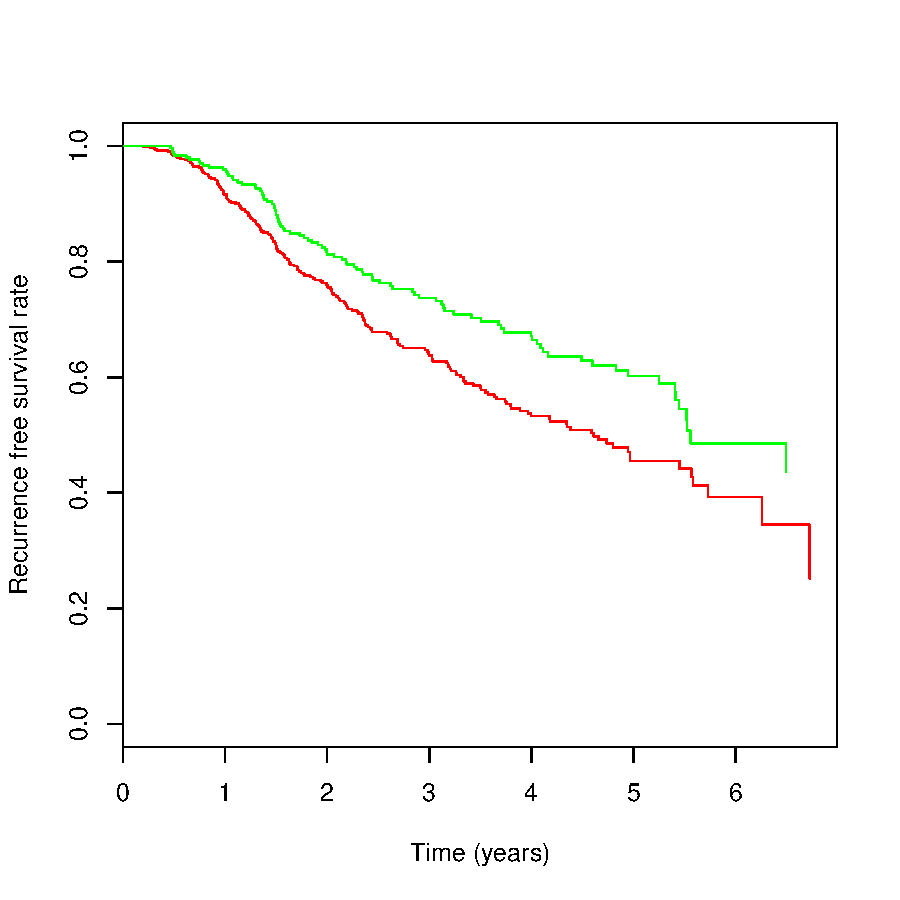
\includegraphics{mfp-FIG1}
\caption{\label{fig1} Predicted survival curves of the final mfp model for the two strata defined by hormonal treatment (red line = no hormonal treatment, green line = hormonal treatment).}
\end{figure}

The function \texttt{plot.mfp} draws three plots: 
smoothed martingale based residuals of the null model, the linear predictor function and a plot of the partial residuals together with a lowess smooth (\ref{fig2}).

\begin{figure}[htb]
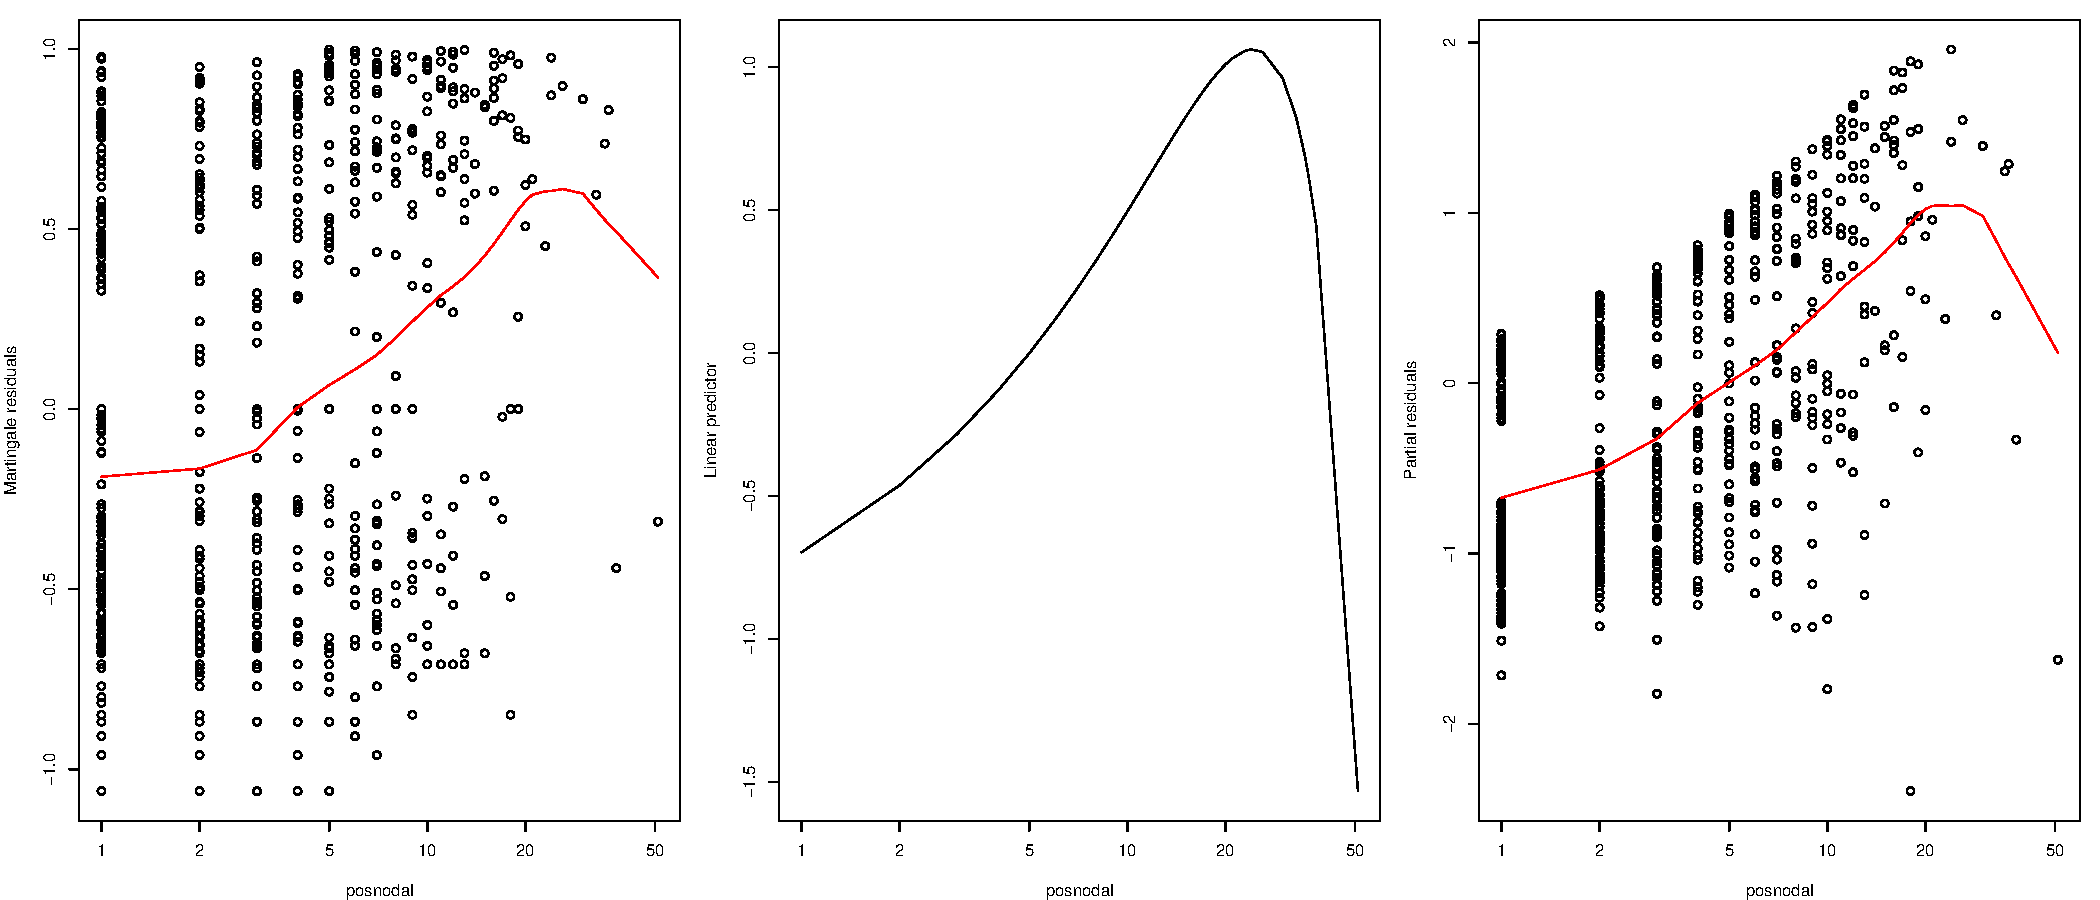
\includegraphics{mfp-FIG2}
\caption{\label{fig2} Smoothed null model martingale residuals, the plot of the estimated 
functional form of the influence of the number of positive lymph nodes ({\tt posnodal}) on the log relative hazard of tumor recurrence, 
and the partial residuals plot for {\tt posnodal}.}
\end{figure}

\addcontentsline{toc}{section}{References}

\bibliographystyle{acm}
\bibliography{mfp}

\end{document}
